Die Abkürzung \emph{GHS/CLP} steht für \emph{Global Harmonized System of 
Classification and Labelling of Chemicals} (Global Harmonisiertes System zur 
Einstufung und Kennzeichnung von Chemikalien) der Vereinten Nationen. Ziel ist 
eine weltweite Angleichung von nationalen und regionalen Systemen. Dies ist 
eine verbindliche Verordnung und muss von allen Unternehmen der chemischen 
Industrie aus den Mitgliedsstaaten der Vereinten Nationen umgesetzt werden. 
Aus der Verordnung ergeben sich die Einführung von neuen Gefahrenpiktogrammen, 
Gefahrenklassen, höheren Einstufungen bekannter Stoffe und Gemische sowie 
Gefahren- und Sicherheitshinweise. \cite{ifag}

\subsection{Gefahrenpiktogramme}

Der Aufbau der Piktogramme ist ein auf der Spitze stehendes weißes Quadrat mit 
rotem Rand und schwarzem Symbol. Der größte Unterschied zu den alten Piktogrammen
ist die einheitliche Färbung aller Piktogramme. Auf der linken Seite der Abbildungen 
\ref{fig:umwgefahren} bis \ref{fig:gesgefahren} sind die alten Piktogramme zu sehen.
\begin{figure}[!ht]
    \centering
    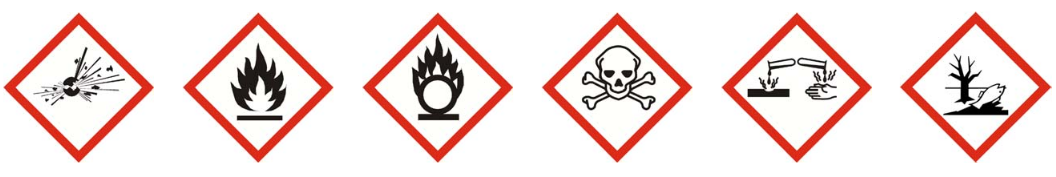
\includegraphics[height=80pt, width=\textwidth]{Piktogramm1.PNG}
    \caption[Piktogramme Teil 1]{\small{Piktogramme Teil 1. \cite{ifaa}}}
    \label{fig:pikto1}
\end{figure}

\noindent
Des Weiteren wurden folgende neue Symbole geschaffen:
\begin{figure}[!ht]
    \centering
    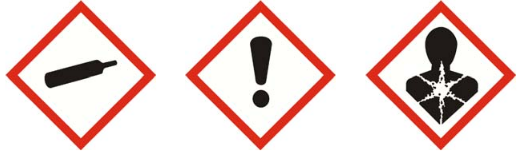
\includegraphics[height=70pt, width=240pt]{Piktogramm2.PNG}
    \caption[Piktogramme Teil 2]{\small{Piktogramme Teil 2. \cite{ifaa}}}
    \label{fig:pikto2}
\end{figure}

\noindent
Unterhalb der Piktogramme müssen, je nach Notwendigkeit, die Signalwörter "'Gefahr"' für 
die gefährlichen Gefahrenkategorien und / oder "'Achtung"' für die weniger 
bedrohlichen Gefahrenkategorien verwendet werden. Ebenso wurden folgende 
Ersetzungsregeln für die Verwendung der Piktogramme definiert \cite{ifaa}:
\begin{itemize}[itemsep=0pt]
    \item Totenkopf ersetzt Ausrufezeichen (bisher: T ersetzt Xn, Xi)
    \item Ätzsymbol ersetzt Ausrufezeichen für Augen- oder Hautreizungen 
    (bisher: C ersetzt Xn, Xi)
    \item Bei Explosion ist Flamme und Brennender Kreis fakultativ, außer es gibt 
    Ausnahmen (bisher: E ersetzt F, O)
    \item Gesundheitsgefahr ersetzt Ausrufezeichen für Hautsensibilisierung oder 
    Haut- und Augenreizung
    \item Regel T ersetzt C - entfällt
\end{itemize}

\noindent
Mit den Abkürzungen \emph{T, Xn, Xi, E, F, O, C} sind die alten Bezeichnungen der Piktogramme 
gemeint, wobei \emph{T} für giftig / sehr giftig, \emph{Xn} und \emph{Xi} für 
gesundheitsschädlich / reizend, \emph{E} für explosionsgefährlich, \emph{F} und \emph{O}
für entzündlich / brandfördernd und \emph{C} für ätzend steht.

\subsection{Gefahrenklassen}

Die Einteilung der Gefahrenklassen besteht aus den folgenden drei Hauptgruppen mit Untergruppen:

\begin{table}[H]
\centering
\begin{tabu} to 1.0\textwidth { | X[l] | } \hline
  \textbf{Physikalische / Chemische Gefahren} \\ [0.5ex] \hline
    Explosive Stoffe/Gemische \& Erzeugnisse mit Explosivstoff \\ \hline
    Entzündbare Gase / Aerosole \\ \hline
    Oxidierende Gase / Flüssigkeiten / Feststoffe \\ \hline
    Gase unter Druck \\ \hline
    Entzündbare Flüssigkeiten / Feststoffe \\ \hline
    Selbstzersetzliche Stoffe und Gemische \\ \hline
    Pyrophore Flüssigkeiten / Feststoffe \\ \hline
    Selbsterhitzungsfähige Stoffe \& Gemische \\ \hline
    Stoffe \& Gemische, die in Berührung mit Wasser entzündbare Gase entwickeln \\ \hline
    Organische Peroxide \\ \hline
    Korrosiv gegenüber Metallen \\ \hline
  \textbf{Gesundheitsgefahren} \\ \hline 
    Akute Toxizität \\ \hline
    Ätz-/ Reizwirkung auf die Haut \\ \hline
    Schwere Augenschädigung / Augenreizung \\ \hline
    Sensibilisierung der Atemwege oder der Haut \\ \hline
    Keimzellmutagenität \\ \hline
    Karzinogenität \\ \hline
\end{tabu}
\end{table}

\begin{table}[H]
\centering
\begin{tabu} to 1.0\textwidth { | X[l] | } \hline
    Reproduktionstoxizität \\ \hline
    Spezifische Zielorgan-Toxizität (einmalige Exposition) \\ \hline
    Spezifische Zielorgan-Toxizität (wiederholte Exposition) \\ \hline
    Aspirationsgefahr \\ \hline
  \textbf{Umweltgefahren} \\ \hline
    gewässerschädigend \\ \hline
    die Ozonschicht schädigend (EU-spezifisch) \\ \hline
\end{tabu}
\end{table}

\subsection{Höhere Einstufung von Stoffen und Gemischen}

Des Weiteren ist eine meist höhere Einstufung bekannter Stoffe und Gemische 
vorzunehmen. Ein Beispiel hierfür ist, dass alle Gasflaschen, auch nicht-explosive 
Gase, zur neuen Gefahrenklasse „Gase unter Druck“ gehören und mit dem 
Gasflaschenpiktogramm gekennzeichnet werden müssen. Atemwegssensibilisierende 
Stoffe werden als gefährlich eingestuft und mit dem Symbol des menschlichen 
Umrisses ausgewiesen. \cite{dguv}

\subsection{Gefahren- und Sicherheitshinweise}

Ebenfalls wurden neue Gefahren- und Sicherheitshinweise geschaffen. Die neuen 
H-Sätze (Hazard Statements) sind wesentlich differenzierter als die alten R-Sätze 
(Risk Statements) und beschreiben Gefährdungen die von chemischen Stoffen 
ausgehen. Es müssen alle zutreffenden H-Sätze verwendet werden. Die neuen P-Sätze 
(Precautionary Statements) ersetzen die S-Sätze (Safety Statements) und geben 
Sicherheitshinweise zu Punkten Allgemeines, Prävention, Reaktion, Lagerung und 
Entsorgung. Auf dem Etikett können bis zu sechs P-Sätze verwendet werden (siehe 
Auflistung der H- und P- Sätze im Kapital \ref{sec:Anhang} - Anhang). \cite{dguv}

\subsection{Kennzeichnungsetikett nach GHS/CLP}

Das Etikett wird in der jeweiligen Amtssprache beschriftet, in dem der Stoff oder 
das Gemisch verkauft wird (mehrere Sprachen sind nicht ausgeschlossen). Das 
Etikett benötigt folgende Informationen \cite{dguv}:
\begin{itemize}[itemsep=0pt]
    \item Herstellerinformationen (Name, Adresse, Telefon) 
    \item Menge des Stoffes oder Gemisches
    \item Produktidentifikation
    \item Gefahrenpiktogramme (wenn vorhanden)
    \item Signalwort (wenn vorhanden)
    \item Gefahrenhinweise (wenn vorhanden)
    \item Sicherheitshinweise (wenn vorhanden)
    \item Ergänzende Informationen (wenn vorhanden)
\end{itemize}

\subsection{Gegenüberstellung alte / neue Einstufung \& Kennzeichnung}

Auf den Abbildungen \ref{fig:umwgefahren} bis \ref{fig:gesgefahren} sieht man die 
Änderungen der Einstufung \& Kennzeichnung nach \emph{GHS/CLP} Verordnung: 

\begin{figure}[H]
    \centering
    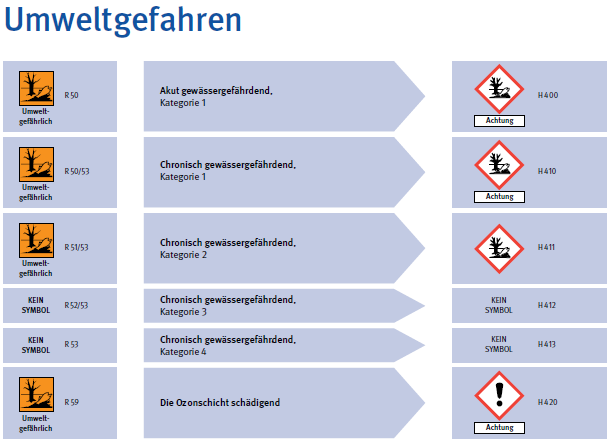
\includegraphics[height=300pt, width=\textwidth]{Gruppe3.PNG}
    \caption[Umweltgefahren]{\small{Umweltgefahren. \cite{bgw}}}
    \label{fig:umwgefahren}
\end{figure}

\begin{figure}[H]
    \centering
    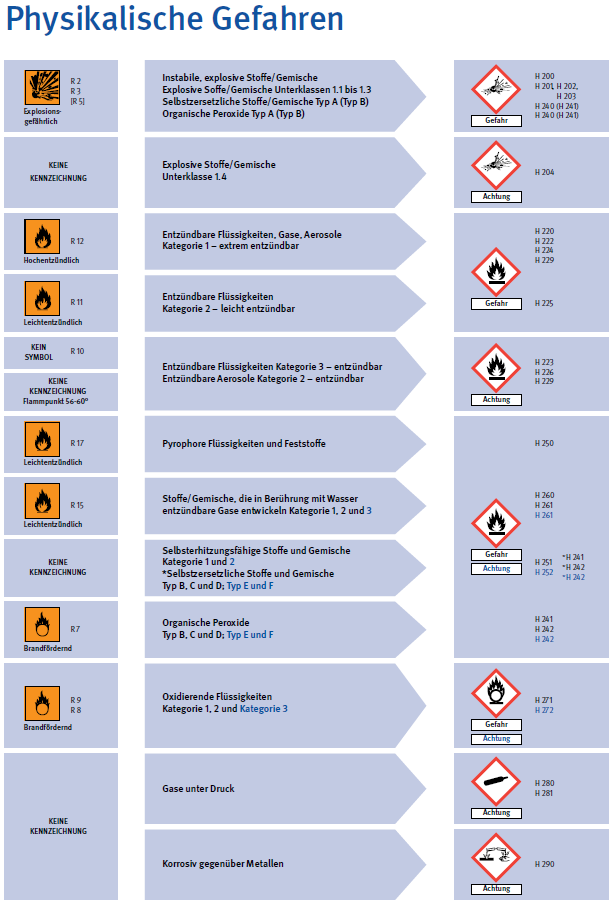
\includegraphics[height=590pt, width=\textwidth]{Gruppe1.PNG}
    \caption[Physikalische Gefahren]{\small{Physikalische Gefahren. \cite{bgw}}}
    \label{fig:phsgefahren}
\end{figure}

\begin{figure}[H]
    \centering
    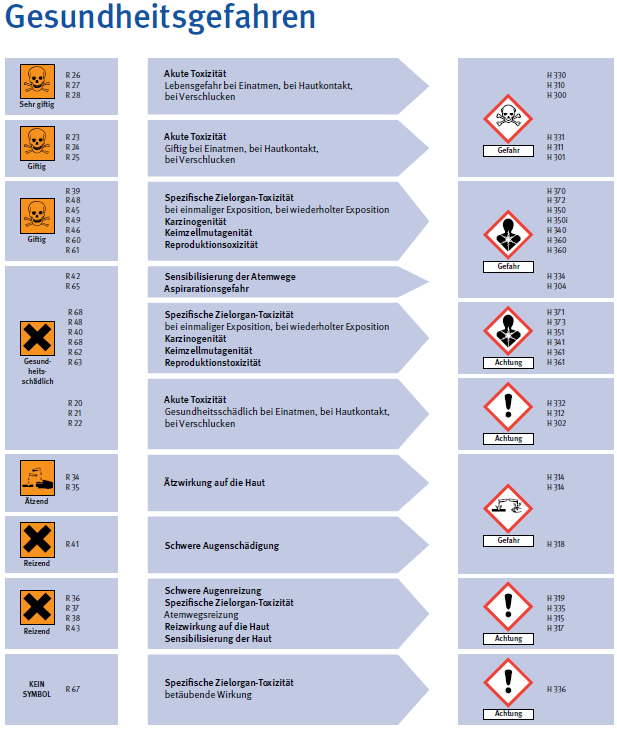
\includegraphics[height=560pt, width=\textwidth]{Gruppe2.PNG}
    \caption[Gesundheitsgefahren]{\small{Gesundheitsgefahren. \cite{bgw}}}
    \label{fig:gesgefahren}
\end{figure}
